\documentclass{article}
\usepackage{lmodern} % Latin Modern Font
\usepackage[T1]{fontenc}
\usepackage{authblk}
\usepackage{amsfonts} % \mathbb
\usepackage[margin=0.5in]{geometry}
\usepackage[utf8]{inputenc}
\usepackage{graphicx}
\usepackage[backend=biber, style=apa]{biblatex}
\usepackage{amsmath}
\usepackage{hyperref}
\usepackage{hypcap}
\DeclareMathOperator{\sign}{sign}
\bibliography{bibli}
\hypersetup{
  colorlinks=true, 
  allcolors=black,
  pdfauthor={Carlos Henrique Tarjano Santos},
  pdftitle={Robust Digital Envelope Estimation Via Geometric Properties of an Arbitrary Real Signal}
}
\title{Robust Digital Envelope Estimation Via Geometric Properties of an Arbitrary Real Signal}
\author[1]{Carlos Henrique Tarjano Santos}
\author[2]{Valdecy Pereira}
\affil[1]{(corresponding author, carlostarjano@id.uff.br) Department of Production Engineering, Universidade Federal Fluminense, Rua Passo da Pátria, 156, Campus Praia Vermelha, Bloco D - sala 309, São Domingos, Niterói, RJ, Brasil, CEP: 24.210-240}
\affil[2]{Department of Production Engineering, Universidade Federal Fluminense, Rua Passo da Pátria, 156, Campus Praia Vermelha, Bloco D - sala 309, São Domingos, Niterói, RJ, Brasil, CEP: 24.210-240}

\begin{document}

\maketitle


\begin{abstract}
Despite being an elusive concept, the temporal amplitude envelope of a signal is essential for its complete characterization, being the primary information-carrying medium in spoken voice and telecommunications, for example. Intuitively, the temporal envelope can be understood as a smooth function that multiplies the signal, being responsible for its outer shape. 
Envelope detection techniques have applications in areas like health, sound classification and synthesis, seismology and speech recognition. Nevertheless, a general method to digital envelope detection of signals with rich spectral content doesn't exist, as most methods involve manual intervention, in the form of filter design, smoothing, as well as other specific design choices, based on a priori knowledge about the nature of the specific waves under investigation.
To address this problem, we propose a framework that uses intrinsic characteristics of a signal to estimate its envelope, completely eliminating the necessity of parameter tuning.
The approach here described draws inspiration from geometric concepts to isolate the frontiers and thus estimate the temporal envelope of an arbitrary signal; to that end, alpha-shapes, concave hulls, and discrete curvature are explored. We also define entities, such as a pulse and frontiers, in the context of an arbitrary digital signal, as a means to reduce dimensionality and the complexity of the proposed algorithm. Specifically, a new measure of discrete curvature is used to obtain the average radius of curvature of a discrete wave, serving as a threshold to identify the wave's frontier points. 
We find the algorithm accurate in the identification of the frontiers of a wide range of digital sound waves with very diverse characteristics, while localizing each pseudo-cycle of the wave in the time domain. The algorithm also compares favourably with classic envelope detection techniques based on filtering and the Hilbert Transform.
Besides the most direct applications of this work to audio classification and synthesis, we foresee impact in compression techniques and machine learning approaches to audio. The discrete curvature definition presented could also be extended to three-dimensional settings, to improve shape detection algorithms based on alpha-shapes.
\end{abstract}

{\bf Keywords:} DSP, alpha-shapes, envelope detection, discrete curvature estimation


\section{Introduction}
Envelope detection is ubiquitous in both analogue and digital signal processing \parencite{2011CaetanoImproved}. Nevertheless, the literature in this area is very fragmented \parencite{2017LyonsDigital}. Besides, most envelope detection techniques are designed to account for very specific settings, like pure sinusoids with moderate noise content, a limitation that excludes most physical signals, as is the case of recorded sound, for example; that limitation arises in part due to the lack of a strict mathematical definition of a temporal envelope \parencite{2013Mengempirical}.

In many natural signals, however, the temporal amplitude envelope of a signal plays a prominent role in the characteristics exhibited: according to \textcite{2017QiRelative}, for example, the envelope is at least as important as the fine structure of a sound wave in the context of the intelligibility of mandarin tones. This is also the case for English \parencite{1995ShannonSpeech}, where even envelopes modulating mostly noise were still capable of conveying meaning. 

The envelope helps to impart emotion and identity to the human voice \parencite{2018ZhuContributions}, and envelope preserving characteristics in concert halls are associated with their pleasantness \parencite{2011LokkiEngaging}.

When dealing with broadband signals, approaches tailored to specific applications are prevalent, such as the one presented by \textcite{2014YangFast} for the distributed monitoring of fibre optic or the one formulated by \textcite{2018AssefModeling} in the context of medical ultrasound imaging.

Addressing the different units in the horizontal and vertical axes, one can transform the DSP problem of envelope detection into the geometric problem of defining the shape of a set of points in $ \mathbb{R}^2 $. For that purpose, \textcite{1983Edelsbrunnershape} introduced the concept of alpha-shapes, a mathematically well-defined extension to the convex hull of a finite set of points, closely related to the Delaunay triangulation and Voronoi diagrams of those points.

This approach is used in areas such as the detection of features in images \parencite{2016VarytimidisAlpha}, reconstruction of surfaces from a cloud of points \parencite{2015WuAutomated} and Spectroscopy \parencite{2019XuModeling}, with the last work, which involves the estimation and removal of the Blaze function (a kind of envelope) of an echelle spectrograph, being particularly illustrative of the potential of cross-fertilization.

Steps in the direction of translating geometric algorithms to the context of envelope detection were also made by \textcite{2015YangSkeleton} via an algorithm based on the construction of a skeleton underlying the wave, and also via the direct translation of computer vision methods to the task \parencite{2015YangRepresenting}.

Following this path, we present a general approach to envelope detection, exploiting the intrinsic characteristics of a generic, spectrally complex wave, in order to avoid the need for manual intervention or parameter tuning.

While the robustness of the proposed approach allows it to be used as a plug-in replacement for many methods encountered in the literature, we feel that it would be particularly useful for sound synthesis.

The envelope is shown to add complexity to the spectral representation of a wave \parencite{2019TarjanoNeuro}, and an accurate description of the envelope, while describing the evolution of the instantaneous amplitude of a signal in time, would also greatly simplify further spectral analysis. Moreover, the algorithm developed in this work naturally divides a signal into its pseudo-cycles, pinpointing them in the time domain, providing the building blocks for the reconstruction of the fine structure of the wave.

The rest of this paper is divided as follows: After explaining and defining the various entities to be used subsequently, of which the concept of frontiers is arguably the most important, in the methodology section, we dedicate a section to present a new discrete curvature estimation approach, and how it was used to identify the frontiers of a discrete wave.

We then proceed to illustrate the results of the application of the algorithm in a set of six diverse sound waves, ranging from voice to unpitched instruments comparing, afterwards, its performance with that of classic digital envelope estimation algorithms, both from a visual and numerical standpoint.

We then discuss the implications of the work, emphasizing the focus on the construction of new interpretations of the relationship between time domain and frequency domain sound descriptions, and our vision of the impact of this methodology in the field of sound synthesis, providing directions for future developments.


\section{Methodology}

In this work it is assumed, without loss of generality, that one is interested in retrieving the mathematically ill-defined \parencite{2013Mengempirical} temporal envelope of an arbitrary physical sound wave, of which only a digital representation is available. 

Naturally, due to the necessary truncations both in time and amplitude, as well as measurement errors introduced by the instruments used to record the signal, it is not possible to exactly recover the original, continuous wave, from its digital counterpart.

The best representation one can hope to get of the original wave is, then, the recording itself. It is sensible, thus, to characterize the envelope of the wave in terms of a subset of the exact samples that comprise its digital representation.

To that end, this work will emphasize the concept of frontier, as the points of the digital wave that mark the wave's upper and lower boundaries; from those points an envelope, conforming to the vague definitions of uniqueness and smoothness, can be trivially constructed, as will be shown.

We start by defining a pulse as a series of consecutive samples of a discrete wave that have the same sign. More formally, let $ W[i] \in \mathbb{R} \ \forall \ i \in \mathbb{N}_0; \ i < n \in \mathbb{N}_0 $ be a real, discrete and finite signal indexed, without loss of generality, over an adjacent subset of the natural numbers starting at zero. This definition relates closely to the concept of an array or vector in most programming languages, and is used in the interest of simplicity.

A pulse $ P[j]; \ \forall \ j \in \mathbb{N}_0; \ j < q \in \mathbb{N}_0; q \le n $ is, then, a subset of $ W $ with cardinality $ \#P[j] = b - a $ such that $ \sign(W[a-1]) \ne \sign(W[a]) = \sign(W[a+1]) = \dots = \sign(W[b-1]) = \sign(W[b]) \ne \sign(W[b+1]) \ \forall \ i; \ a \le i \le b; \ a, b \in \mathbb{N}_0 $.

In other words, each pulse is a unique subset of $ W $ with its members being the maximum sequence of samples of $ W $ having the same signal. Thus $ P[0] \cup P[1] \cup \cdots \cup P[q-1] = W $ and $ P[i_1] \cap P[i_2] = \emptyset \ \forall \ i_1, i_2 \in \mathbb{N}_0;\ i_1 \ne i_2; \ i_1, i_2 < q $.

Naturally, each pulse can be classified as positive ($ P[j]^+ $) or negative ($ P[j]^- $), based on the sign of its samples, which must be the same. It is also convenient to attribute to each pulse a pair of coordinates: those will be the coordinates of the sample with the maximum absolute amplitude in each pulse, and will be denoted by $ P[j]^\pm_x $ and $ P[j]^\pm_y $. Additionally, the length, or cardinality, of a pulse will be denoted by $ \#P[j]^\pm $.

For an arbitrary continuous function, then, a pulse would correspond to the regions between its roots; for a sinusoid, a pulse would be equal to half of its cycle. In analogy, two consecutive pulses, naturally with opposing signs, have the potential to delimitate a pseudo-cycle, as illustrated in figure \ref{fig:Pulses}. For that to be true, however, the pulses need to make part of the frontiers of the signal, as yet to be defined.

  \begin{figure}[ht!]
    \centering
      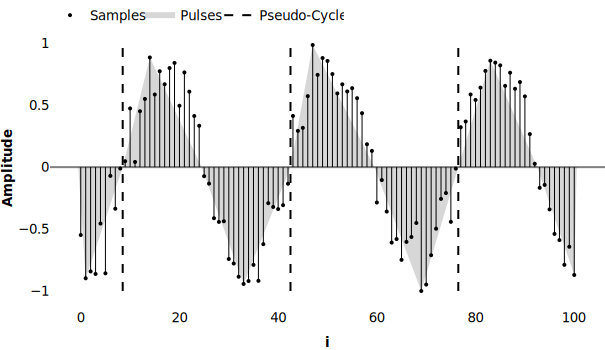
\includegraphics[width=0.8\linewidth]{01Pulses.pdf}
    \caption{Example of a discrete wave. The black stems represent the individual samples of the signal. The grey areas encompass the simplified convex hulls of the pulses. The dashed lines mark the frontiers between pseudo-cycles.}
    \label{fig:Pulses}
  \end{figure}

The most mathematically sound definition of an envelope involves the representation of its underlying wave as an analytic signal, introduced by Gabor in 1946 \parencite{2007HahnHistory}. In his work, \textcite{1946GaborTheory} applies the then relatively new mathematical machinery of the quantum mechanics to unify the time and frequency representations of a wave, showing how the Hilbert transform could be applied to a real signal in order to obtain an equivalent complex signal, later known as the analytic signal.

This analytic signal has the form $ a(t) = s(t) + \mathbb{H}(s(t)) \ \text{i} $ \parencite{2016HePraat} where $ s(t) $ is the original real signal. $ \mathbb{H}(s(t)) $, the Hilbert transform of the original signal, becomes the imaginary part of the analytic signal; the envelope of a signal thus represented can be straightforwardly obtained by the computation of its complex modulus.

Figure \ref{fig:AnalyticSignal} shows the envelope obtained via the analytic signal, for a pure sinusoid with a local frequency of 20 cycles, modulated by a polynomial of the third degree, illustrating the difference in the shape of the envelope in the presence and absence of gaussian white noise with standard deviation of $ 1/10 $ of the wave's maximum amplitude.

\begin{figure}[ht!]
  \centering
    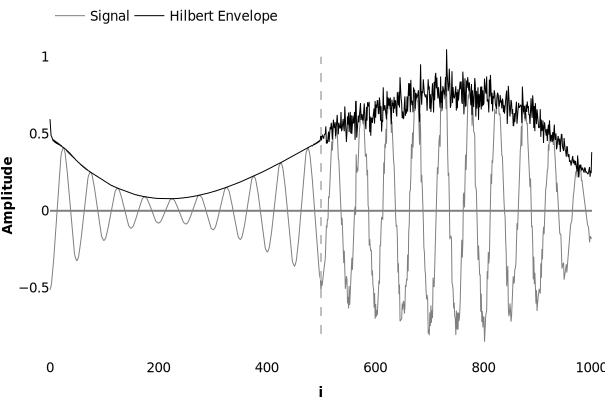
\includegraphics[width=0.8\linewidth]{02AnalyticSignal.pdf}
  \caption{Envelope of a pure sinusoid modulated by a polynomial of degree 3, as obtained by the Hilbert Transform. In the first half, the sinusoid is free of noise, while in the second half white gaussian noise with a standard deviation of $ 1/10 $ of the maximum amplitude of the wave was added to the base signal.}
  \label{fig:AnalyticSignal}
\end{figure}

It is readily noticeable from figure \ref{fig:AnalyticSignal} that, as soon as noise is introduced in the original signal, it is reflected in the envelope, breaking our assumption of smoothness. Other than that, this definition yields a unique, positive envelope.

In practice, however, is not uncommon for a discrete wave, especially in the case of sound, to present somewhat different positive and negative contours; to account for this discrepancy, we will define a positive (upper) and a negative (lower) frontier of a discrete wave. They will be composed by the points $ (i, W[i]) $ that are, necessarily but not sufficiently, the points of respectively maximum and minimum amplitude of their pulses, i.e. $ (P[j]^\pm_x, P[j]^\pm_y) $.

The set of all these points such that $ W[i] > 0 $ will be called the positive, piecewise linear frontier and will be denoted by $ F^+ $. Similarly, $ F^- $ will denote the negative frontier of $ W $, defined by the subset of points $ (i, W[i]) $ where $ W[i] < 0 $, as is shown in figure \ref{fig:Frontiers}. 

\begin{figure}[ht!]
  \centering
    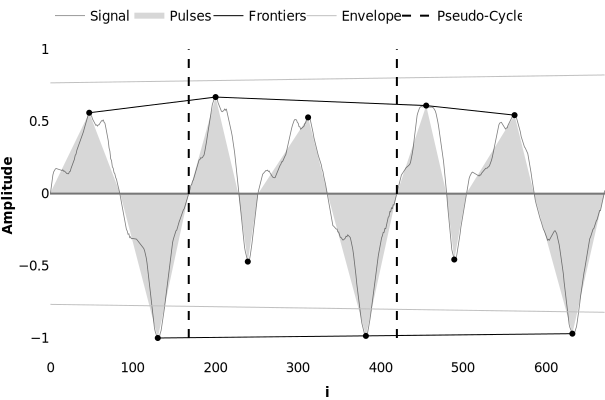
\includegraphics[width=0.8\linewidth]{03Frontiers.pdf}
  \caption{Positive and negative frontiers, envelope and pseudo-cycles for a fragment of piano sound. While we have only one (positive) envelope, here mirrored in the inferior space, we have two frontiers, the superior and inferior, that are obtained independently.}
  \label{fig:Frontiers}
\end{figure}

To identify such points, we need first to address the different units in which the amplitude and horizontal distance of our wave are expressed. To make abscissa and ordinate units consistent for the computation of the frontiers, and proceed with a geometric treatment of the subject, we consider the set of positive and negative pulses separately. 

For each set, we multiply all pulses vertical coordinates by the average length of the pulses in the set, after having divided by the average of the pulses' amplitudes, putting both axes in the same unit $i$, related to time by the equation $i = t \ \mathit{fps}$.

Formally, supposing we have $ m $ pulses of the same sign, we scale each pulse's vertical coordinate $ P[j]^\pm_y $ by $ s^\pm $, where:

\begin{equation} \label{eq:scale}
  s^\pm = \frac{\sum_{j=1}^{m} \#P[j]^\pm}{\sum_{j=1}^{m} P[j]^\pm_y}
\end{equation}

Because we are interested in approximating a function that is smooth over the whole domain of the wave, we can assume that, in the scale of a pulse, this function will be very close to a horizontal straight line and, thus, won't touch any point inside the convex hull defined by the pulse. 

By the same token, as the change in amplitude from one pulse to the next pulse with the same sign is motivated by changes in this same envelope, one can reasonably suppose that $ \max(P[j]) \approx \max(P[j+2]) $.

This makes clear that only one point of an arbitrary pulse can be in the frontier, namely, its point of maximum amplitude; those definitions will allow us to derive the frontiers of a wave using an alpha-shapes inspired algorithm without the need to compute the Delaunay triangulation first.

That also justifies the approximation of the convex hull of a pulse by the triangle defined by the points where the pulse crosses the horizontal axis and the point of maximum amplitude $ (P[j]^\pm_x, P[j]^\pm_y) $; this triangular pulse and, more specifically, its point of maximum, will become the atomic unit for the rest of the method.

Translating the intuitive explanation of alpha-shapes in \textcite{1994EdelsbrunnerThree} to our context, we can say that the points in the frontier are those touched by a circle of a given radius $ r $ outside the signal that is not allowed to contain any point of the signal; the pulses that contain said points can be seen as frontier pulses.

Intuitively, one can picture a circle being rolled above (or below, in the case of the negative frontier) the signal, and marking the points it touches as frontier points.

We can now revisit the concept of a pseudo-cycle, only hinted at before, defining it as the samples of the original wave that belong to two successive pulses that, in turn, belong to their respective frontiers, including eventual pulses between them, as can be seen in figure \ref{fig:Frontiers}.

It is necessary to infer the appropriate radius $ r $ of such a circle and, to that end, a measure of the curvature of a discrete function is needed. Discrete curvature estimation is an important task in image processing \parencite{2010FleischmannNovel} for which no default definition exists. 

The two possible general approaches are the derivation of direct methods that use characteristics of the discrete wave to calculate the curvature, or the use of the smooth curvature of a curve fitted to the discrete wave \parencite{2001CoeurjollyDiscrete}.

Concerning the last method, two approaches to fit a polynomial to a generic wave are readily available: the least mean squares approach, that seeks to minimize the dependent variable errors and the total least squares problem, that treats both variables symmetrically \parencite{1980GolubAnalysis}.

The geometric, symmetrical nature of the problem excludes the more computationally economic least mean squares approach, however, leaving us with the total least squares, for which no general closed-form solutions are available \parencite{2007MarkovskyOverview}; this leads us to turn our attention to direct approaches of curvature estimation.


\subsection{Discrete Curvature Estimation - The Equivalent Circle Approach}

As previously noted, no default discrete curvature definition exists; \textcite{2014CarrollSurvey}, for example, derive three such different definitions based on the approximation of a circle by an inscribed, centred and circumscribed polygon. In the context of 3d meshes, \textcite{2016VasaMultivariate} evaluate a range of existing estimators from a multivariate point of view.

None of those approaches, especially for being defined over the vertices of a discrete wave, fit seamlessly into our algorithm; we thus proceed to define a discrete curvature measure over the edges of a discrete wave. To that end we are going to apply the definition of smooth curvature as the rate of change of the unit tangent to a curve, noting that this is equivalent to that of the osculating circle \parencite{2016VasaMesh}.

The idea is to find the equivalent circle whose tangent presents the same change in direction, in the same horizontal distance, as the edge of interest, as shown in figure \ref{fig:DiscreteCurvature}.

\begin{figure}[ht!]
  \centering
    
\includegraphics[width=0.2\linewidth]{04DiscreteCurvature.pdf}
  \caption{The tangent unit vector of the circle changes from the horizontal direction in $ \hat{u}_0 $ to an inclination of $ \theta $ in $ \hat{u}_1 $. $ \theta $ is also the angle between the average direction $ \vec{\overline{v}}_l $ and the vector $ \vec{v}_l $ that represents the edge of interest, shown in grey.}
  \label{fig:DiscreteCurvature}
\end{figure}

For each frontier, the angle $ \theta $ between the average direction and each of the vectors can be obtained via the relation between the slopes $ d $ of the respective lines, as in the expression $ \theta = \arctan( (d - \overline{d}) / (1 + d \overline{d}) ) $, with $\overline{d} = \sum_{l=1}^{m-1} (P[l+1]_y - P[l]_y) / (P[l+1]_x - P[l]_x) $ and $ d_l = (P[l+1]_y - P[l]_y)/ (P[l+1]_x - P[l]_x) $

The radii of the equivalent circles are thus given by $ r_l = x_l / \sin (\theta_l) $ with the curvature given by $\kappa_l = 1/r_l=\sin (\theta_l) / x_l$, where $ x_l = P[l+1]_x - P[l]_x $ and $ y_l = P[l+1]_y - P[l]_y $. Joining both equations, one can write:

\begin{equation} \label{eq:radius}
  r_l = \left\lvert \frac{x_l \sqrt{\overline{d}^2 + 1} \ \sqrt{x_l^2 + y_l^2}}{\overline{d} x_l - y_l} \right\rvert
\end{equation}

After this procedure, illustrated in figure \ref{fig:Curvatures}, two sets of points in $ \mathbb{R}^2 $, corresponding to the positive and negative frontiers, are obtained, where the ordinates represent the instantaneous radius, with its localization in the time domain given by the abscissas. 

\begin{figure}[ht!]
  \centering
    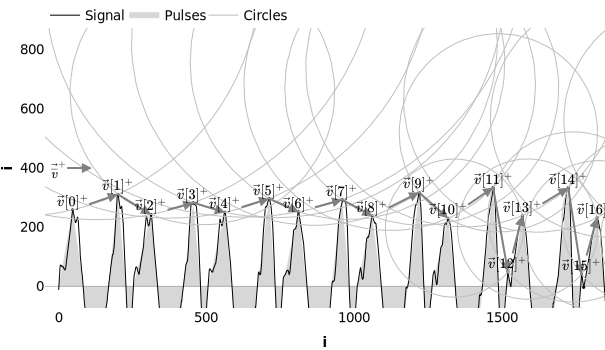
\includegraphics[width=0.8\linewidth]{05Curvatures.pdf}
  \caption{The equivalent circles obtained via the procedure described for the positive frontier. $\theta$, the angle between $ \vec{\overline{v}}^+$ and each of the $\vec{v}_l^+$ is used, as is the horizontal component of each $\vec{v}_l^+$ to obtain the radii of the circles.}
  \label{fig:Curvatures}
\end{figure}

Given the robustness of the method, for an average wave of a few seconds at an ordinary rate of 44100 $ \mathit{fps} $ the average of the radius values is sufficient to assure the accurate identification of the frontier. However, a curve fitting method can be used in the case of longer or ill-behaved waves. 
An example of the use of the average equivalent circle can be seen in figure \ref{fig:AvgCircle}.

\begin{figure}[ht!]
  \centering
    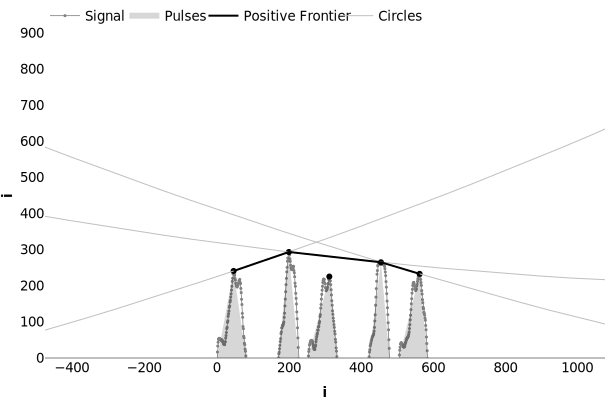
\includegraphics[width=0.8\linewidth]{06AvgCircle.pdf}
  \caption{The positive frontier as obtained by the use of the circle representing the average curvature of the discrete wave illustrated.}
  \label{fig:AvgCircle}
\end{figure}

\section{Results}

Figure \ref{fig:FullFrontiers} illustrates the frontiers of six diverse discrete sound waves, as well as an in-detail view of the highlighted segment for each signal. All waves are records of physical sounds, chosen to represent the applicability of the algorithm in real-world scenarios.

\begin{figure}[ht!]
  \centering
    
\includegraphics[width=0.8\linewidth]{07FullFrontiers.pdf}
  \caption{Positive and negative frontiers of six digital waves, as extracted by the algorithm here presented. For each wave, the region highlighted in black is shown in detail besides the whole wave. For each wave the horizontal axis is the sample number $i$, while the vertical axis is the normalized amplitude. All 6 waves were recorded at 44100 $ \mathit{fps} $.}
  \label{fig:FullFrontiers}
\end{figure}

We can see that the frontier is satisfactorily detected in the case of harmonic and inharmonic sounds, and is robust in relation to the number of samples and the frequencies of the waves.

The impact of the normalization of a wave using the frontiers obtained can be seen in figure \ref{fig:Fourier}, which shows the original and normalized wave in the case of a recording of the key 33 of a piano both in the time and frequency domains. We can see that the Fourier power spectra is greatly simplified in the case of the normalized wave.

\begin{figure}[ht!]
  \centering
    \includegraphics[width=0.8\linewidth]{08Fourier.pdf}
  \caption{Original and normalized views of a recording of key 33 (F3, 175 Hz) from a grand piano both in time and frequency domains.}
  \label{fig:Fourier}
\end{figure}

\subsection{Robustness}

Figures \ref{fig:xRobustness} and \ref{fig:yRobustness} illustrate the computational resilience of the algorithm for scaling in both the abscissa and ordinate axes, respectively. This is due to the normalization scheme presented in equation \ref{eq:scale}.

Although important from a theoretical standpoint, this step has an especial computational relevance in the case of digital sound waves, as they tend to be composed of a high number of samples with relatively low amplitudes, generally normalized between -1 and 1, leading to a numerical disparity between axes.

\begin{figure}[ht!]
  \centering
    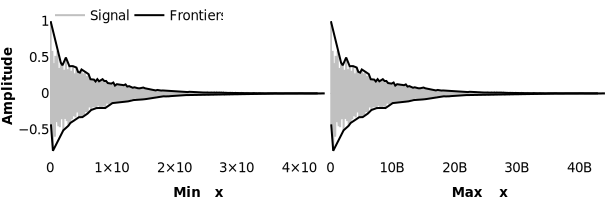
\includegraphics[width=0.8\linewidth]{10xRobustness.pdf}
  \caption{Minimum and maximum scales of the abscissa before computational stability issues arose, for a recording of a drum kit tom.  $ \text{B} = 10^6 $.}
  \label{fig:xRobustness}
\end{figure}

\begin{figure}[ht!]
  \centering
    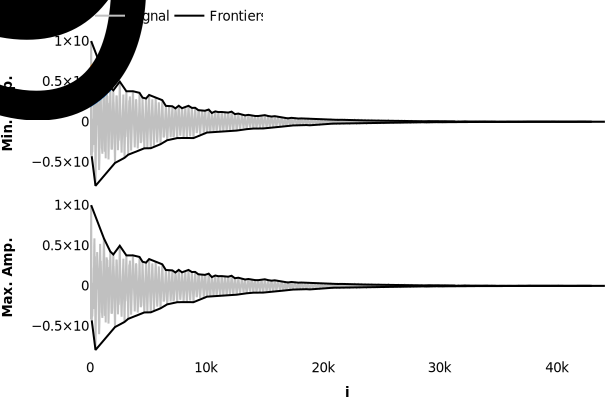
\includegraphics[width=0.8\linewidth]{09yRobustness.pdf}
  \caption{Minimum and maximum values of the amplitude before computational stability issues arose, for a recording of a drum kit tom.}
  \label{fig:yRobustness}
\end{figure}

\subsection{Comparison with traditional algorithms}

Direct comparison with many of the more recent algorithms is made difficult by the unavailability of digital implementations of such works, many designed to process analogue signals \parencite[e.g.,][]{2018AssefModeling}.

Nevertheless, insight can be gained from a comparison of the results of the method here proposed with some of the most common envelope extraction algorithms, as can be seen in figure \ref{fig:Comparison}.

\begin{figure}[ht!]
  \centering
    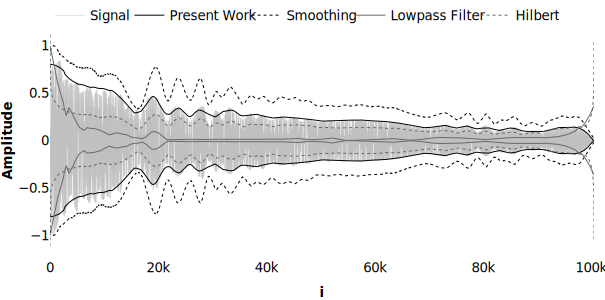
\includegraphics[width=0.8\linewidth]{12Comparison.pdf}
  \caption{Comparison of the algorithm present in this work with the most common methods of digital envelope identification.}
  \label{fig:Comparison}
\end{figure}

For a recording of a guitar sound, in which a bend is performed, we contrast the proposed algorithm with four common approaches of varying complexity: simple smoothing of the rectified original wave, low pass filtering followed by rectification, peak identification and subsequent smoothing, and the extraction of the envelope via Hilbert transform, as presented earlier in the paper, with a previous smoothing of the original wave to avoid the artifacts shown in figure \ref{fig:AnalyticSignal}.

All those methods demanded careful choice of parameters: in the case of filtering, a cut-off frequency of approximately 88 Hz was used, consisting of one additional parameter to be tuned. For all the other traditional approaches, the Savitzky-Golay smoothing algorithm was used, and the window size was the parameter to be defined.

In the case of the proposed algorithm, the smooth temporal envelope was obtained merging both positive and negative frontiers, the result being smoothed with the same procedure described. Figure \ref{fig:FrontiersToEnvelope} illustrates the results.

\begin{figure}[ht!]
  \centering
    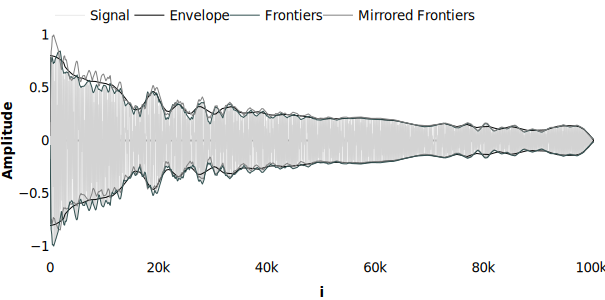
\includegraphics[width=0.8\linewidth]{13FrontiersToEnvelope.pdf}
  \caption{Original positive and negative frontiers in dark grey and their mirrored versions. The temporal envelope, in black, is obtained by merging and approximating both frontiers.}
  \label{fig:FrontiersToEnvelope}
\end{figure}

Table \ref{table:Comparison} presents a computational comparison between the techniques. The times are for custom implementations of those methods in the Python programming language. The least mean squares result was calculated by halving the envelopes presented in figure \ref{fig:Comparison} and comparing them with the rectified absolute wave, so as to avoid the potential influence of an estimated frequency. 

We can see that, while the algorithm here presented is the most accurate, it's also the most computationally intensive. The connection between alpha-shapes and Delaunay triangulation can be explored in future works as a means to improve the efficiency of the algorithm.

\begin{table}[ht!]
\centering
\begin{tabular}{ l c c }
\hline
Method & LMS & time(s) \\
\hline
Presented Algorithm & 0.0088 & 4.1507 \\ 
Smoothing           & 0.0123 & 0.1911 \\ 
Low pass Filter      & 0.0258 & 0.5601 \\ 
Hilbert Transform   & 0.0141 & 0.2599 \\ 
\hline
\end{tabular}
\caption{Comparison of the algorithm present in this work with the most common methods of digital envelope identification.}
\label{table:Comparison}
\end{table}

\subsection{Retrieving information about the underlying wave}

The algorithm provides the position of the pseudo-cycles of a wave, with which one can, for example, derive its fundamental frequency and phase: using one of the two frontiers, we have $ f = (\#F^\pm - 1) n / (F^\pm[-1] - F^\pm[0])$, where $ \#F^\pm $ denotes the cardinality of the frontier, while $ F^\pm[0] $ and $ F^\pm[-1] $ stand for the frontier's first and last item, respectively.

Similarly, each point of each of the frontiers can be used to estimate the local phase at that location. For the positive frontier, it is necessary to note that, for each point, the following equation holds: $ \cos(\phi + 2 \pi f i / n) = 1 $, and thus $ \phi = 2 \pi k - 2 \pi f i / n $, with $ k \in \mathbb{N} $, while for the negative frontier $ \cos(\phi + 2 \pi f i / n) = -1 $ and $ \phi = 2 \pi k + \pi - 2 \pi f i / n) $.


\section{Discussion}

This work hopes to fill a gap identified by the authors in the context of sound synthesis, where the lack of procedures for the accurate identification of the temporal envelope of arbitrary waves consists of an obstacle to the complete description and eventual manipulation of signals.

While relevant in its own accord, the procedure here presented isolates the individual pseudo-cycles of a wave, pinpointing them in the time domain. Due to that, a rich set of theoretical advancements, of whose an example was given in the end of the preceding section, can be built upon this initial algorithm.

With the knowledge of the exact position and characteristics of the pseudo-cycles of a wave, one can investigate its evolution in time, in terms of waveform, for example, free from the potential interference of a modulating wave; in other words, one can have a very satisfactory view of the instantaneous shape and phase of an arbitrary wave and its evolution in time, providing a way to bridge the gap between time domain and frequency domain interpretations.

In the context of sound synthesis, for example, one would be able to apply specific methods for the recreation of the envelope, more in line with its smooth, slow varying and non-periodic nature and a different approach to the periodic and relatively fast changes of the temporal fine structure.


\subsection{Conclusion}

It is our opinion that such theoretical advances can be used in the formulation of better representations of discrete sounds, that in turn can improve sound compression techniques, while providing more adequate representation for the application of machine learning techniques for both sound classification and synthesis.

\section{References}

\printbibliography[heading=none]

\end{document}
